\section{Nonexcluded regions in the pMSSM parameter space}

\label{sec:unexplored}
Of the 7200 pMSSM points considered in this study, about 3700 cannot be
excluded by CMS analyses based on their $Z$-significance (Fig.~\ref{fig:Z} (d)), although more
than half of these nonexcluded points have a total cross section greater than 10 fb at $\sqrt{s}$ = 8~\TeV.
Given this unexpected result, it is of interest to characterize this nonexcluded
subspace in order to shed light on why the CMS analyses are not
sensitive to these points, which can help guide the design of future analyses. To this end, we decompose the nonexcluded subspace into the dominant physical processes and
follow with an idealized analysis of final state
observables.

\begin{figure}[h]
\centering
%\renewcommand*\thesubfigure{\arabic{subfigure}}
\hspace{0mm}
  \makebox[.21\textwidth][c]{
        \setlength{\unitlength}{\linewidth}
        \begin{picture}(.21,.21)
         \put(0,0){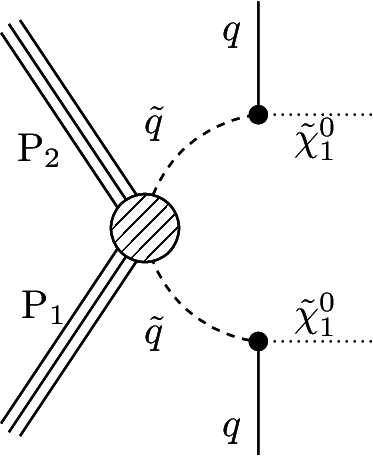
\includegraphics[width=.21\unitlength]{figures/pMSSMpaper/topologies/1_T2qq.png}}
         \put(0.11,-0.015){\makebox(0,0){\small (1) $\tilde{\rm q}\tilde{\rm q}(\tilde{\rm q} \hspace{-1mm}\rightarrow \hspace{-1mm}{\rm q}\tilde{\chi}_{1}^{0})$}}
        \end{picture}
}
\hspace{0mm}
  \makebox[.21\textwidth][c]{
        \setlength{\unitlength}{\linewidth}
        \begin{picture}(.21,.21)
         \put(0,0){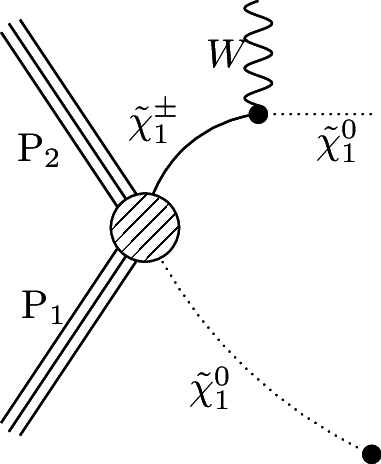
\includegraphics[width=.21\unitlength]{figures/pMSSMpaper/topologies/2_C1qq.png}}
         \put(0.11,-0.015){\makebox(0,0){\small (2) $\tilde{\chi}^{\pm}_{1}\tilde{\chi}^{0}(\tilde{\chi}^{\pm}_{1} \hspace{-1mm}\rightarrow \hspace{-1mm}{\rm W}^{\pm}\tilde{\chi}_{1}^{0})$}}
        \end{picture}
}
\hspace{0mm}
  \makebox[.21\textwidth][c]{
        \setlength{\unitlength}{\linewidth}
        \begin{picture}(.21,.21)
         \put(0,0){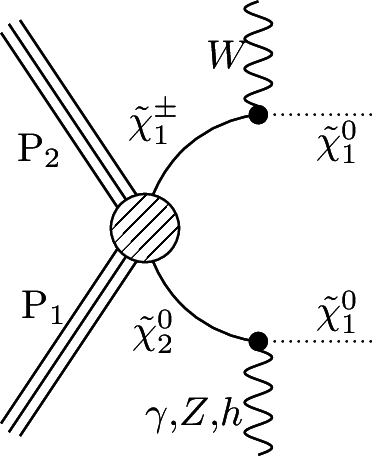
\includegraphics[width=.21\unitlength]{figures/pMSSMpaper/topologies/3_TChiWB.png}}
         \put(0.11,-0.015){\makebox(0,0){\small (3) $\tilde{\chi}^{\pm}_{1}\tilde{\chi}^{0}_{2}(\tilde{\chi} \hspace{-1mm}\rightarrow \hspace{-1mm}{\rm V/h}\tilde{\chi}_{1}^{0})$}}
        \end{picture}
}
\hspace{0mm}
  \makebox[.21\textwidth][c]{
        \setlength{\unitlength}{\linewidth}
        \begin{picture}(.21,.21)
         \put(0,0){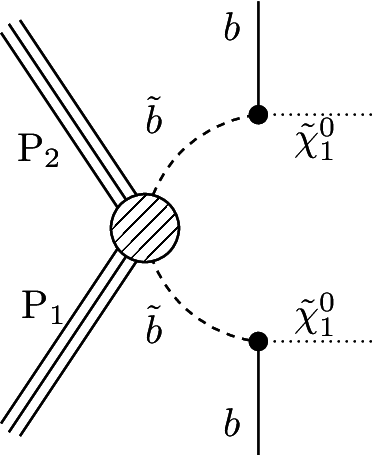
\includegraphics[width=.21\unitlength]{figures/pMSSMpaper/topologies/4_T2bb.png}}
         \put(0.11,-0.015){\makebox(0,0){\small (4) $\tilde{\rm b}\tilde{\rm b}(\tilde{\rm b} \hspace{-1mm}\rightarrow \hspace{-1mm}{\rm b}\tilde{\chi}_{1}^{0})$}}
        \end{picture}
}
\centering
\vspace{1.5cm}
\hspace{0mm}
  \makebox[.21\textwidth][c]{
        \setlength{\unitlength}{\linewidth}
        \begin{picture}(.21,.21)
         \put(0,0){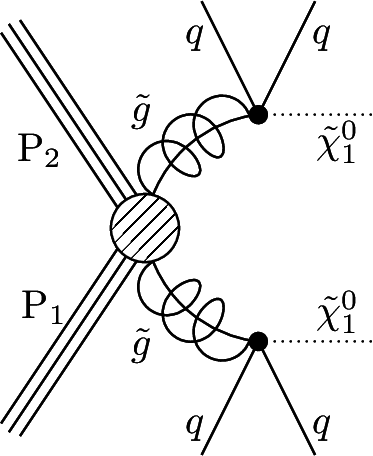
\includegraphics[width=.21\unitlength]{figures/pMSSMpaper/topologies/5_T1.png}}
         \put(0.11,-0.015){\makebox(0,0){\small (5) $\tilde{\rm g}\tilde{\rm g}(\tilde{\rm g} \hspace{-1mm}\rightarrow \hspace{-1mm}{\rm qq}\tilde{\chi}_{1}^{0})$}}
        \end{picture}
}
\hspace{0mm}
  \makebox[.21\textwidth][c]{
        \setlength{\unitlength}{\linewidth}
        \begin{picture}(.21,.21)
         \put(0,0){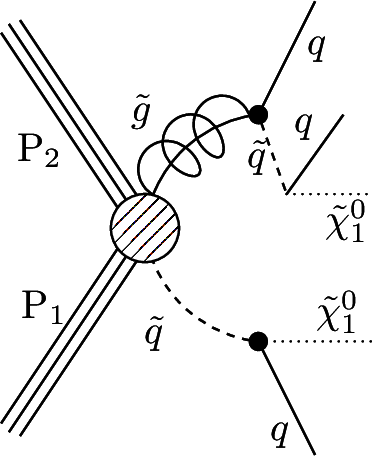
\includegraphics[width=.21\unitlength]{figures/pMSSMpaper/topologies/6_T3qqq.png}}
         \put(0.11,-0.015){\makebox(0,0){\small (6) $\tilde{\rm g}\tilde{\rm q}(\tilde{\rm g} \hspace{-1mm}\rightarrow \hspace{-1mm}\tilde{\rm q}{\rm q}\tilde{\chi}_{1}^{0})$}}
        \end{picture}
}
\hspace{0mm}
  \makebox[.21\textwidth][c]{
        \setlength{\unitlength}{\linewidth}
        \begin{picture}(.21,.21)
         \put(0,0){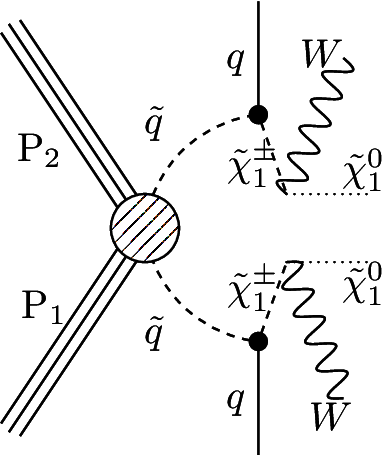
\includegraphics[width=.21\unitlength]{figures/pMSSMpaper/topologies/7_T4qqww.png}}
         \put(0.11,-0.015){\makebox(0,0){\small (7) $\tilde{\rm q}\tilde{\rm q}(\tilde{\rm q} \hspace{-1mm}\rightarrow \hspace{-1mm}{\rm q}\tilde{\chi}^{\pm}_{1})^{\text{*}}$}}
        \end{picture}
}
\hspace{0mm}
 \makebox[.21\textwidth][c]{
        \setlength{\unitlength}{\linewidth}
        \begin{picture}(.21,.21)
         \put(0,0){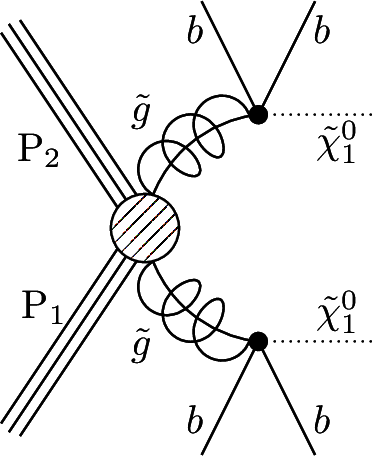
\includegraphics[width=.21\unitlength]{figures/pMSSMpaper/topologies/8_T1bb.png}}
         \put(0.11,-0.015){\makebox(0,0){\small (8) $\tilde{\rm g}\tilde{\rm g}(\tilde{\rm g} \hspace{-1mm}\rightarrow \hspace{-1mm}{\rm bb}\tilde{\chi}_{1}^{0})$}}
        \end{picture}
}
\centering
\vspace{1.5cm}
\hspace{0mm}
 \makebox[.21\textwidth][c]{
        \setlength{\unitlength}{\linewidth}
        \begin{picture}(.21,.21)
         \put(0,0){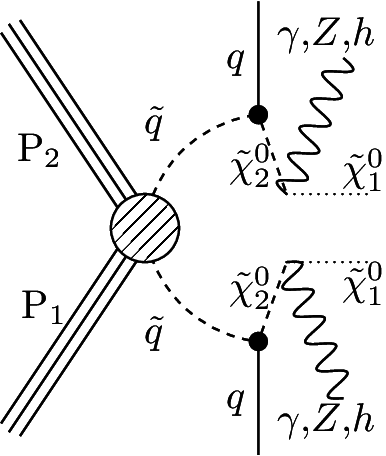
\includegraphics[width=.21\unitlength]{figures/pMSSMpaper/topologies/9_T4zz.png}}
         \put(0.11,-0.015){\makebox(0,0){\small (9) $\tilde{\rm q}\tilde{\rm q}(\tilde{\rm q} \hspace{-1mm}\rightarrow \hspace{-1mm}{\rm q}\tilde{\chi}^{0}_{2})^{\text{*}}$}}
        \end{picture}
}
\hspace{0mm}
 \makebox[.21\textwidth][c]{
        \setlength{\unitlength}{\linewidth}
        \begin{picture}(.21,.21)
         \put(0,0){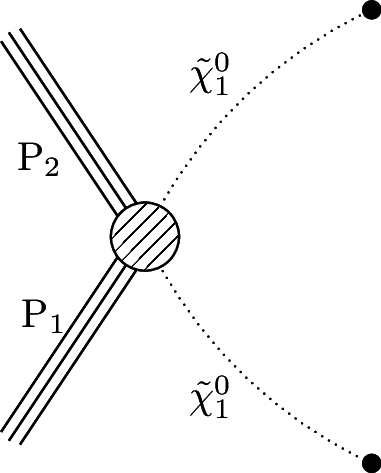
\includegraphics[width=.21\unitlength]{figures/pMSSMpaper/topologies/10_NN.png}}
         \put(0.11,-0.015){\makebox(0,0){\small (10) $\tilde{\chi}^{0}_{1}\tilde{\chi}^{0}_{1}$}}
        \end{picture}
}
\hspace{0mm}
 \makebox[.21\textwidth][c]{
        \setlength{\unitlength}{\linewidth}
        \begin{picture}(.21,.21)
         \put(0,0){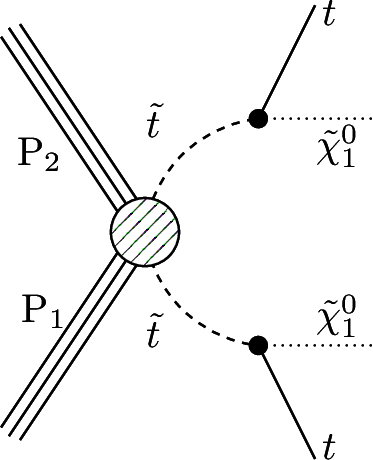
\includegraphics[width=.21\unitlength]{figures/pMSSMpaper/topologies/11_T2tt.png}}
         \put(0.11,-0.015){\makebox(0,0){\small (11) $\tilde{\rm t}\tilde{\rm t}(\tilde{\rm t} \hspace{-1mm}\rightarrow \hspace{-1mm}{\rm t}\tilde{\chi}_{1}^{0})$}}
        \end{picture}
}
\hspace{0mm}
\makebox[.21\textwidth][c]{
        \setlength{\unitlength}{\linewidth}
        \begin{picture}(.21,.21)
         \put(0,0){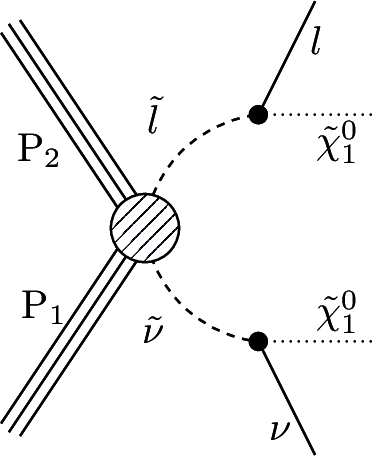
\includegraphics[width=.21\unitlength]{figures/pMSSMpaper/topologies/12_LSnu.png}}
         \put(0.11,-0.015){\makebox(0,0){\small (12) $\tilde{\rm l}^{\pm}\tilde{\nu}(\tilde{\rm l} \hspace{-1mm}\rightarrow
\hspace{-1mm}{\rm l}\tilde{\chi}_{1}^{0})$}}
        \end{picture}
}
\vspace{6 mm}
\caption{The twelve most common principal processes in the pMSSM, listed in order 
of their frequency before the constraints of the CMS searches. Both on-shell and off-shell states are included.
 Indices of particle charge, flavor, and chirality are ignored in the construction, with the exception of the flavor of the third-generation squarks and quarks. Asterisks in the labels indicate where process names involving long decay chains have been abbreviated.}
\label{fig:diagrams1}
\end{figure}


For the decomposition, signal events are analyzed at the generator
level for each model point, and the pair of SUSY particles most frequently produced directly
from the proton-proton interaction is taken as the production 
mode for that model point. Then the principal (dominant) process for
that point is built as a tree diagram starting from the pair of SUSY mother
particles and following the decay modes with the highest branching
fractions until endpoints consisting of only SM particles
and LSPs are reached. Indices of particle charge, flavor,  and chirality are ignored in the
construction, with the exception of the flavor of the third-generation squarks and quarks.
Over 100 distinct principal processes are found
among the total 7200 studied points, of which the first twelve
are listed in Fig.~\ref{fig:diagrams1}. Many
of the principal processes are seen to correspond to common SMS scenarios, while others
depict more unusual scenarios with long decay chains. 

\begin{figure}[h]
  \centering
  \makebox[.647\textwidth][c]{
        \setlength{\unitlength}{\linewidth}
        \begin{picture}(.647,.647)
         \put(0,0){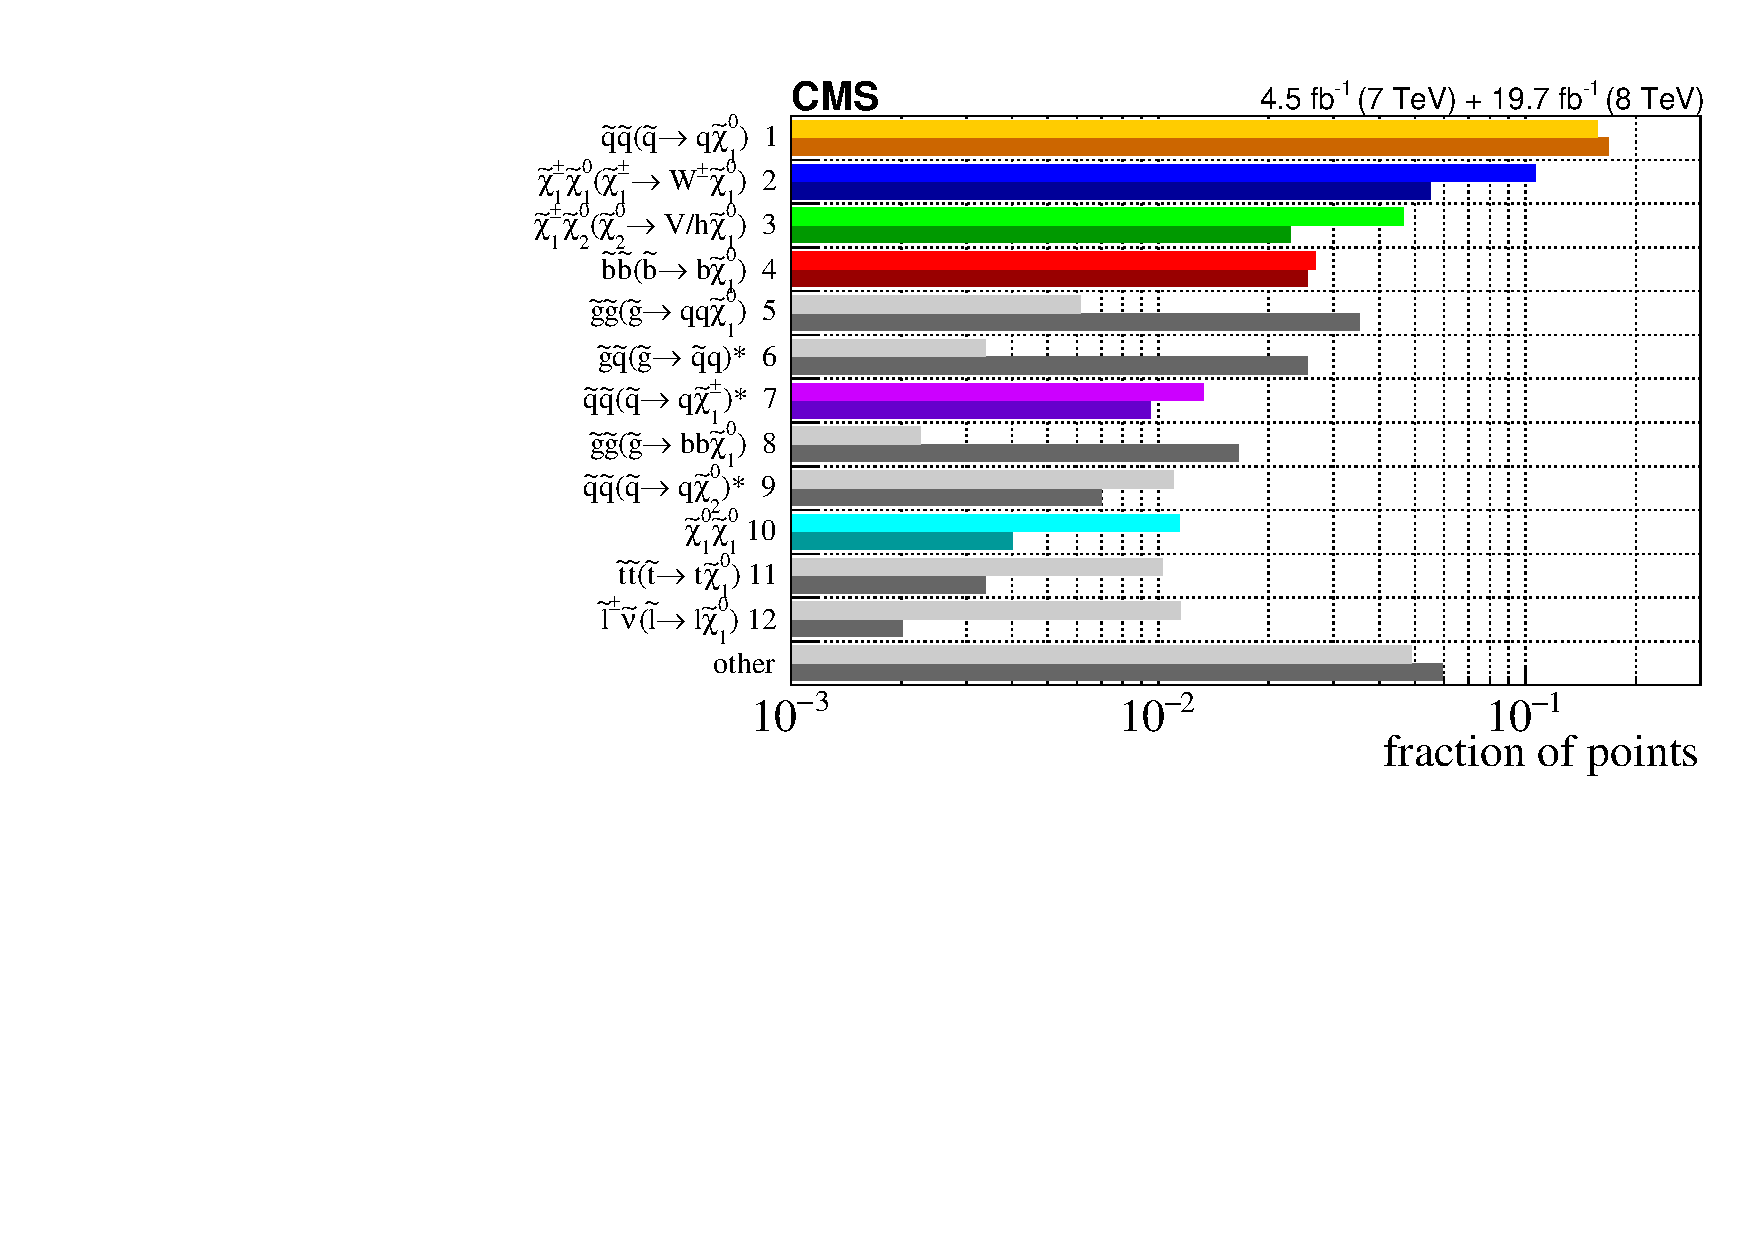
\includegraphics[width=.647\unitlength]{figures/pMSSMpaper/topologies/PrincipalProcesses.pdf}\label{fig:TopoHistoA}}
         \put(0.375,-.0){\scriptsize (a)}
        \end{picture}
}
  \makebox[.344\textwidth][c]{
        \setlength{\unitlength}{\linewidth}
        \begin{picture}(.344,.344)
         \put(0,0){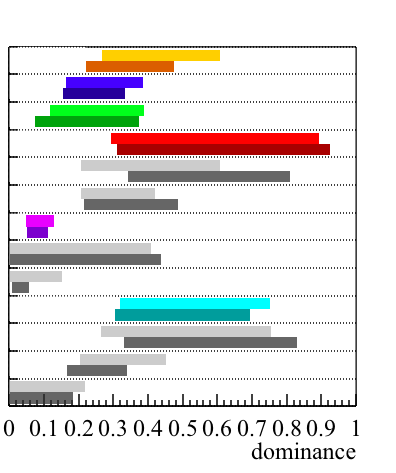
\includegraphics[width=.344\unitlength]{figures/pMSSMpaper/topologies/Dominance.png}\label{fig:TopoHistoB}}
         \put(0.145,-.0){\scriptsize (b)}
        \end{picture}
        }
    \caption{(a) shows the fraction of excluded
  (dark) and nonexcluded (light) points out of all considered points,
  by principal process. Color is assigned to the processes that are most common after the constraints of the CMS searches, which are selected for further study. The dominance
  of principal processes, as defined in Eq.~\ref{eq:dominance}, is given in (b) where the bands show the
  RMS range of the dominance. }
    \label{fig:TopoHisto}
\end{figure}

The distribution of principal processes for excluded and nonexcluded
points is given in Fig.~\ref{fig:TopoHisto} (a).  It is seen that processes
involving direct gluino production (5 and 8) are excluded with
a much higher
frequency than they survive, and those with EW
gaugino production (2, 3, and 10) survive with a higher frequency than they are
excluded. Processes with first-generation squark production (1 and 7) survive
and are excluded at similar rates, and processes with
slepton production (12) have exceptionally high survival rates. 
These trends are likely attributable to the difference in the
production cross section between colored and noncolored particles for
a given SUSY mass scale. 
The overflow bin (other), which contains many principal
processes, including modes of colored and noncolored particle
production, indicates a survival rate approximately equal to the
exclusion rate.  
The dominance is defined for each model point
as the ratio of the cross section of the principal process to the total SUSY
production cross section at 8~\TeV, 
 \begin{equation}
  {\rm dominance} \equiv \sigma^{8~\TeV~}_{\rm principal}/\sigma^{8~\TeV~}_{\rm tot},
  \label{eq:dominance}
\end{equation}
and is shown in Fig.~\ref{fig:TopoHisto} (b). Most values of the dominance are in the
range 0.05\textendash0.60. The excluded and nonexcluded values for the
dominance are seen to agree within the RMS of the distributions, indicating that the
presence of multiple event signatures within a single model
hypothesis does not
significantly impact our ability to exclude such a model point.

Dedicated searches exist that correspond to some of the most frequent principal processes, indicating areas where the SMS approach is likely well optimized. For example, points with principal processes 1, $\tilde{\rm q}\tilde{\rm q}(\tilde{\rm q} \hspace{-1mm}\rightarrow \hspace{-1mm}{\rm q}\tilde{\chi}_{1}^{0})$, and 4, $\tilde{\rm b}\tilde{\rm b}(\tilde{\rm b} \hspace{-1mm}\rightarrow \hspace{-1mm}{\rm b}\tilde{\chi}_{1}^{0})$, enjoy searches that target these processes explicitly.   A few principal processes have not been explicitly targeted by the host of CMS SUSY searches, including processes 2, $\tilde{\chi}^{\pm}_{1}\tilde{\chi}^{0}(\tilde{\chi}^{\pm}_{1} \hspace{-1mm}\rightarrow \hspace{-1mm}{\rm W}^{\pm}\tilde{\chi}_{1}^{0})$, and 3, $\tilde{\chi}^{\pm}_{1}\tilde{\chi}^{0}_{2}(\tilde{\chi} \hspace{-1mm}\rightarrow \hspace{-1mm}{\rm V/h}\tilde{\chi}_{1}^{0})$, the asymmetric EW gaugino production modes. New searches that target these or the other overlooked processes may serve to broaden the overall sensitivity to the pMSSM.

Next, we characterize the nonexcluded model space by the predicted
final states in order to shed light on what signatures may serve to target the nonexcluded points in Run 2.  We define a set of loose baseline physics objects and event 
variables, at the generator level, as follows:
\begin{itemize}
\item Leptons: electrons, muons, or taus having a transverse momentum $p_{\rm T}$ greater than 5 GeV and an isolation less than 0.2. Here, isolation  =
$[(\Sigma_{i}{p_{\rm T}}_i) - p_{\rm T}]/\Sigma_{i}{p_{\rm T}}_i$,
where the sums run over all detector-visible particles $i$ within a
$\Delta$R cone of 0.5 around the object, with $\Delta$R = $\sqrt{(\Delta\eta)^2+(\Delta\phi)^2}$, where $\eta$ is the pseudorapidity and $\phi$ is the azimuthal angle in radians;
%\item Photons: photons having a $p_{\rm T}$ greater than 5\GeV and an isolation less than 0.2, with the same definition of isolation as for leptons;
\item Jets: particles clustered with the anti-kT jet algorithm \cite{Cacciari:2008gp} with distance parameter 0.5. The jets are required to have a $p_{\rm T}$ greater than 20 GeV;
\item b-jets: jets matched to a b hadron within a $\Delta$R of 0.5;
\item \MET{}: the missing transverse energy, calculated as the magnitude
  of the vector sum of the transverse momenta of
 visible particles with $p_{\rm T} >$ 5 GeV; 
\item \HT{}: the scalar sum of the $p_{\rm T}$ of the jets with
  a $p_{\rm T}>$ 50GeV.
%\item MHT: the scalar sum of the transverse momenta of the jets with a $p_{\rm T}>$ 30\GeV
%\item $\Delta \phi($MHT$, jet_{1})$: The average azimuthal separation between the leading jet and the 
%missing \HT{} for events with at least three 50\GeV jets and no isolated leptons or photons.
\end{itemize}

Hi, We use a parallel coordinates visualization technique that enables the
display of multiple dimensions (as introduced in Chapter \ref{chap:SM}). In Fig.~\ref{fig:parcor},
we show nonexcluded points corresponding to the six selected
principal processes (those denoted by color in Fig.~\ref{fig:parcor}).
Vertical axes are chosen to represent meaningful properties of the model
points, and each model point is represented as a curved line traversing the plot from left to right, intersecting each axis at the parameter value taken by the model point. The curvature of the lines is added to help distinguish between similar pMSSM points, but the trajectories of the lines between the axes do not carry physical information. A number of distinct scenarios are seen to have survived the CMS
analyses.  A minimum threshold of 20 fb has been applied to the 8~\TeV~ signal
cross sections to limit the scope to those
points that could potentially still be probed with the Run 1 data set
using an expanded set of analyses and techniques.


\begin{figure}[h]
  \centering
         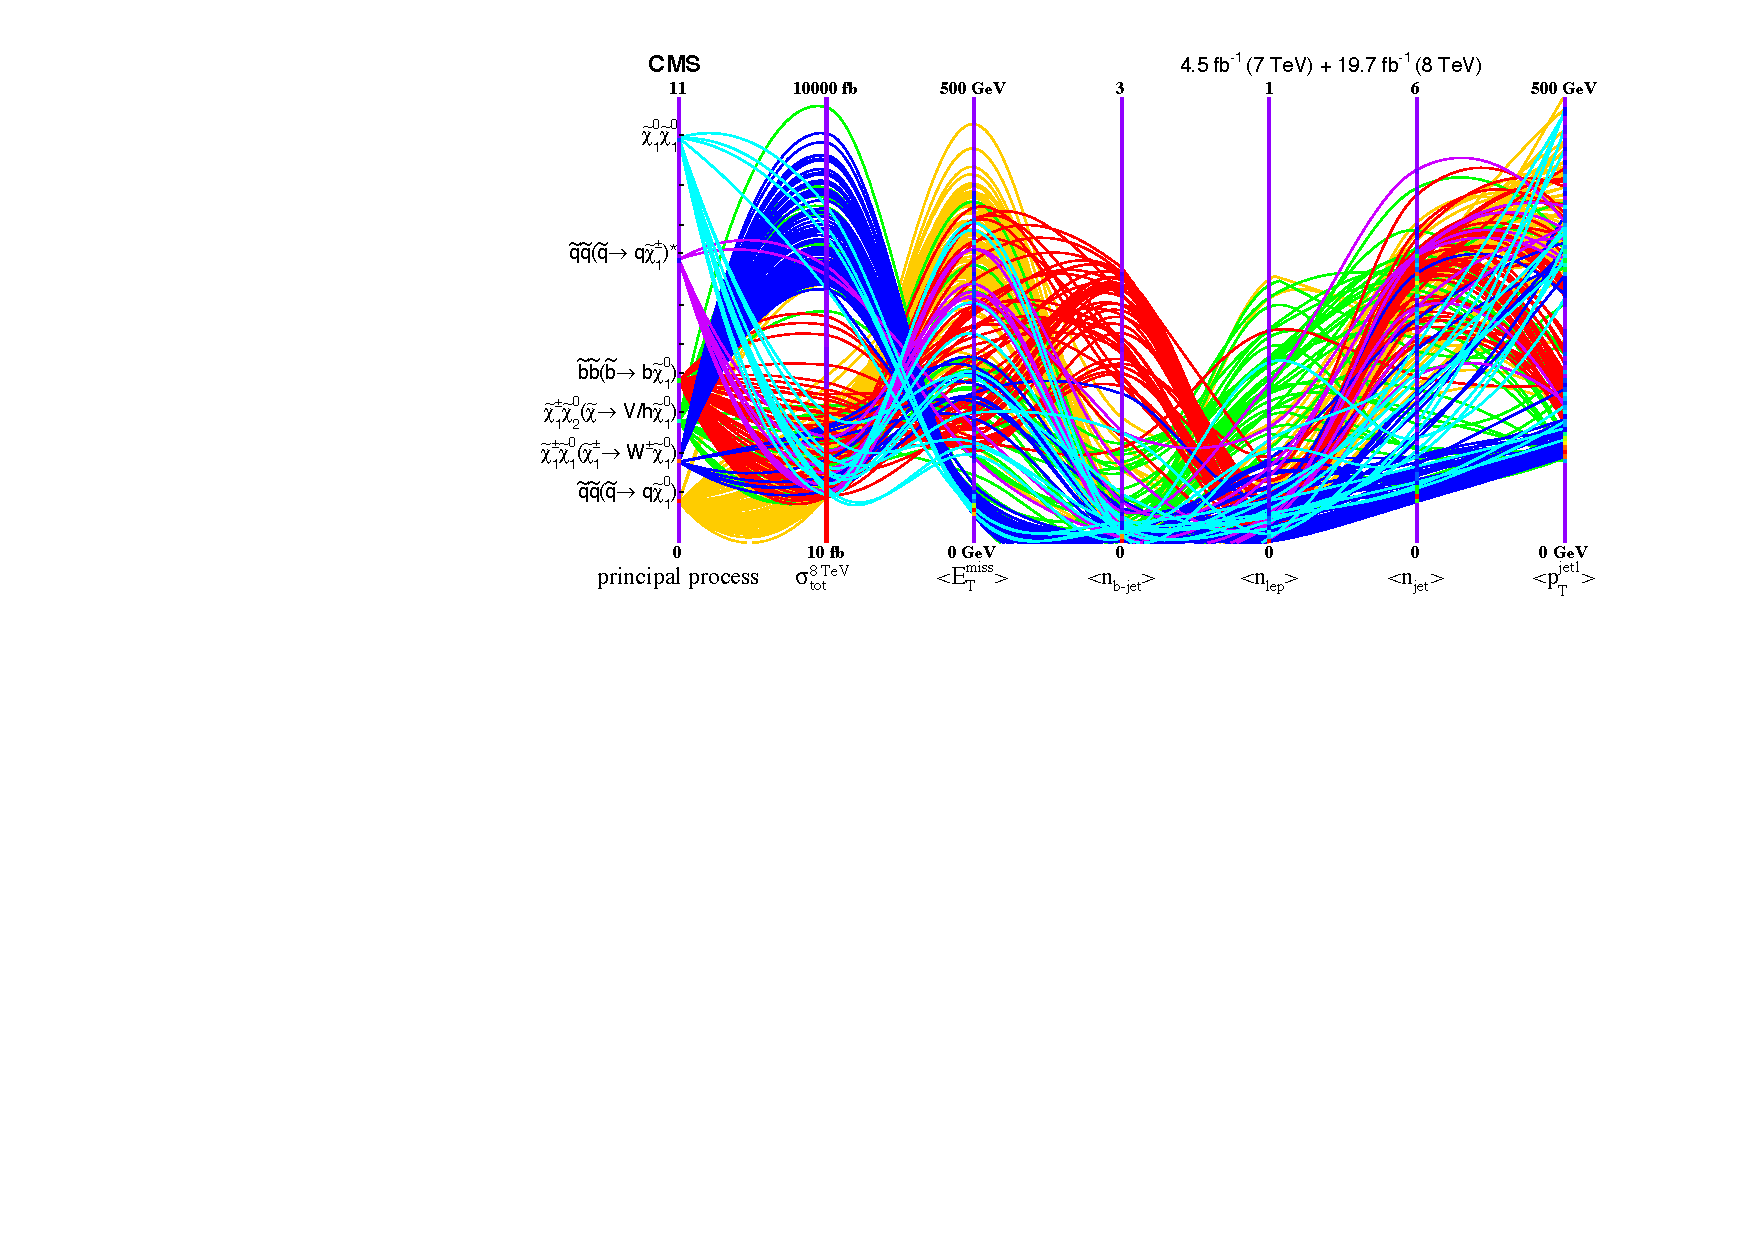
\includegraphics[width=1.0\linewidth]{figures/pMSSMpaper/parallel_coordinates/ParCorTopos.pdf}
    \caption{A parallel coordinates plot showing several hundred
      selected nonexcluded model points for the six most common
      principal processes, with seven key properties.
      From the left, the selected properties are: the principal
      process, the 8~\TeV~ signal production cross section (in
      log$_{\text{10}}$ scale), the average value of the \MET{}, the average number of
      b-jets, leptons, and jets, and finally, the average $p_{T}$
      momentum of the leading jet. Color is assigned based on the
      principal process. Orange codes for process 1, blue for
      process 2, green for 3, red for 4, violet for 7, and 
      cyan for 10.  Lines
      arching toward higher vertical positions typically indicate more
      ``discoverable'' scenarios. }
    \label{fig:parcor}
\end{figure}


The nonexcluded points associated with principal processes 1, $\tilde{\rm q}\tilde{\rm q}(\tilde{\rm q} \hspace{-1mm}\rightarrow \hspace{-1mm}{\rm q}\tilde{\chi}_{1}^{0})$, and 4, $\tilde{\rm b}\tilde{\rm b}(\tilde{\rm b} \hspace{-1mm}\rightarrow \hspace{-1mm}{\rm b}\tilde{\chi}_{1}^{0})$, are seen to give rise to large average \MET{}, jet multiplicities between 2 and 4, and moderate to low cross sections due the the large masses of the squarks. Given the
higher cross sections in Run 2, these high \MET{} scenarios will become increasingly more accessible.

Model points with principal processes 2, $\tilde{\chi}^{\pm}_{1}\tilde{\chi}^{0}(\tilde{\chi}^{\pm}_{1} \hspace{-1mm}\rightarrow \hspace{-1mm}{\rm W}^{\pm}\tilde{\chi}_{1}^{0})$, and 3, $\tilde{\chi}^{\pm}_{1}\tilde{\chi}^{0}_{2}(\tilde{\chi} \hspace{-1mm}\rightarrow \hspace{-1mm}{\rm V/h}\tilde{\chi}_{1}^{0})$, typically predict large cross sections, in the range 100 fb\textendash1 pb, 
but a limited number of physical observables, primarily due to compression in the mass spectrum between the LSP and the other EW gauginos. These points peak low in the average multiplicity of jets, leptons, and in average \MET{}. They could potentially be probed with searches that involve events with initial state radiation and soft boson decay products that are aligned with the \MET{}.

Points with principal processes 3, $\tilde{\chi}^{\pm}_{1}\tilde{\chi}^{0}_{2}(\tilde{\chi} \hspace{-1mm}\rightarrow \hspace{-1mm}{\rm V/h}\tilde{\chi}_{1}^{0})$, and 10, $\tilde{\chi}^{0}_{1}\tilde{\chi}^{0}_{1}$, tend to follow the trend profiled
by process 2, $\tilde{\chi}^{\pm}_{1}\tilde{\chi}^{0}(\tilde{\chi}^{\pm}_{1} \hspace{-1mm}\rightarrow \hspace{-1mm}{\rm W}^{\pm}\tilde{\chi}_{1}^{0})$, differing primarily in the lepton multiplicity and, in the case of at least one lepton, in the average $\pt$ of the highest-$\pt$ lepton (leading lepton). The close resemblance of
processes 10 and 2  is mostly due to the fact that the mass
difference between the $\tilde{\chi}_{1}^\pm$ and
$\tilde{\chi}_1^0$ is frequently very small (less than 1 GeV), causing the ensuing off-shell W 
boson of process 2 to produce undetectably soft particles.

Points with principal processes 5, $\tilde{\rm g}\tilde{\rm g}(\tilde{\rm g} \hspace{-1mm}\rightarrow \hspace{-1mm}{\rm qq}\tilde{\chi}_{1}^{0})$, and 6, $\tilde{\rm g}\tilde{\rm q}(\tilde{\rm g} \hspace{-1mm}\rightarrow \hspace{-1mm}\tilde{\rm q}{\rm q}\tilde{\chi}_{1}^{0})$, the most frequent modes
involving gluinos, are not highlighted in Fig.~\ref{fig:parcor}, since their frequency among nonexcluded points is relatively small. We note that several of the nonexcluded models with very light gluino masses (less than 700 GeV) correspond to principal process 6, with mass differences between the $\tilde{\text{g}}$ and LSP that range around 100~\GeV. Sensitivity to these model points may be possible by considering final states with three or fewer jets and \MET{} thresholds that are lower than typically applied.

Points with principal process 7, $\tilde{\rm q}\tilde{\rm q}(\tilde{\rm q} \hspace{-1mm}\rightarrow \hspace{-1mm}{\rm q}\tilde{\chi}^{\pm}_{1})^{\text{*}}$, do not display distinct trends in the
properties selected, which is partly due to these points having a
low dominance of around 0.1. Such model points have a diverse set of
secondary processes, which are not directly examined here.

A general observation about the model points in Fig.~\ref{fig:parcor}
is the significant anticorrelation of observables, which
manifests as the criss-crossing of lines between the axes. For example,
model points with very high average \MET{} tend to have very low cross sections,
and vice versa. This is a consequence of the fact that, having observed no significant excess of events in data,
the surviving model points are those with very few experimentally accessible 
observables, or they would have been excluded.

With over 50\%
of all nonexcluded points corresponding to cross sections of
greater than 10 fb, it is critical to further examine why these points were not accessed in Run 1.  
We attempt to gain an
understanding by further characterizing the signal, evaluating fiducial cross sections corresponding to a
range of final-state observables. The fiducial cross section
$\sigma_{\text{f}}$ of a final-state is defined for each model point as 
 \begin{equation}
   \sigma_{\text{f}} = \sigma_{\text{tot}}^{\text{8 TeV}}A,
\end{equation}
where {\it A} is the acceptance times signal efficiency
computed as the fraction of simulated signal events
passing a set of event-level criteria. 
We examine a set of final-state observables that loosely correspond to trigger thresholds or
signal regions of the examined searches. Figures
\ref{fig:parcorMET}-\ref{fig:parcorBJet1} show the impact of adjusting
various thresholds on the fiducial cross sections of nonexcluded points.
\begin{figure}[h]
  \centering
         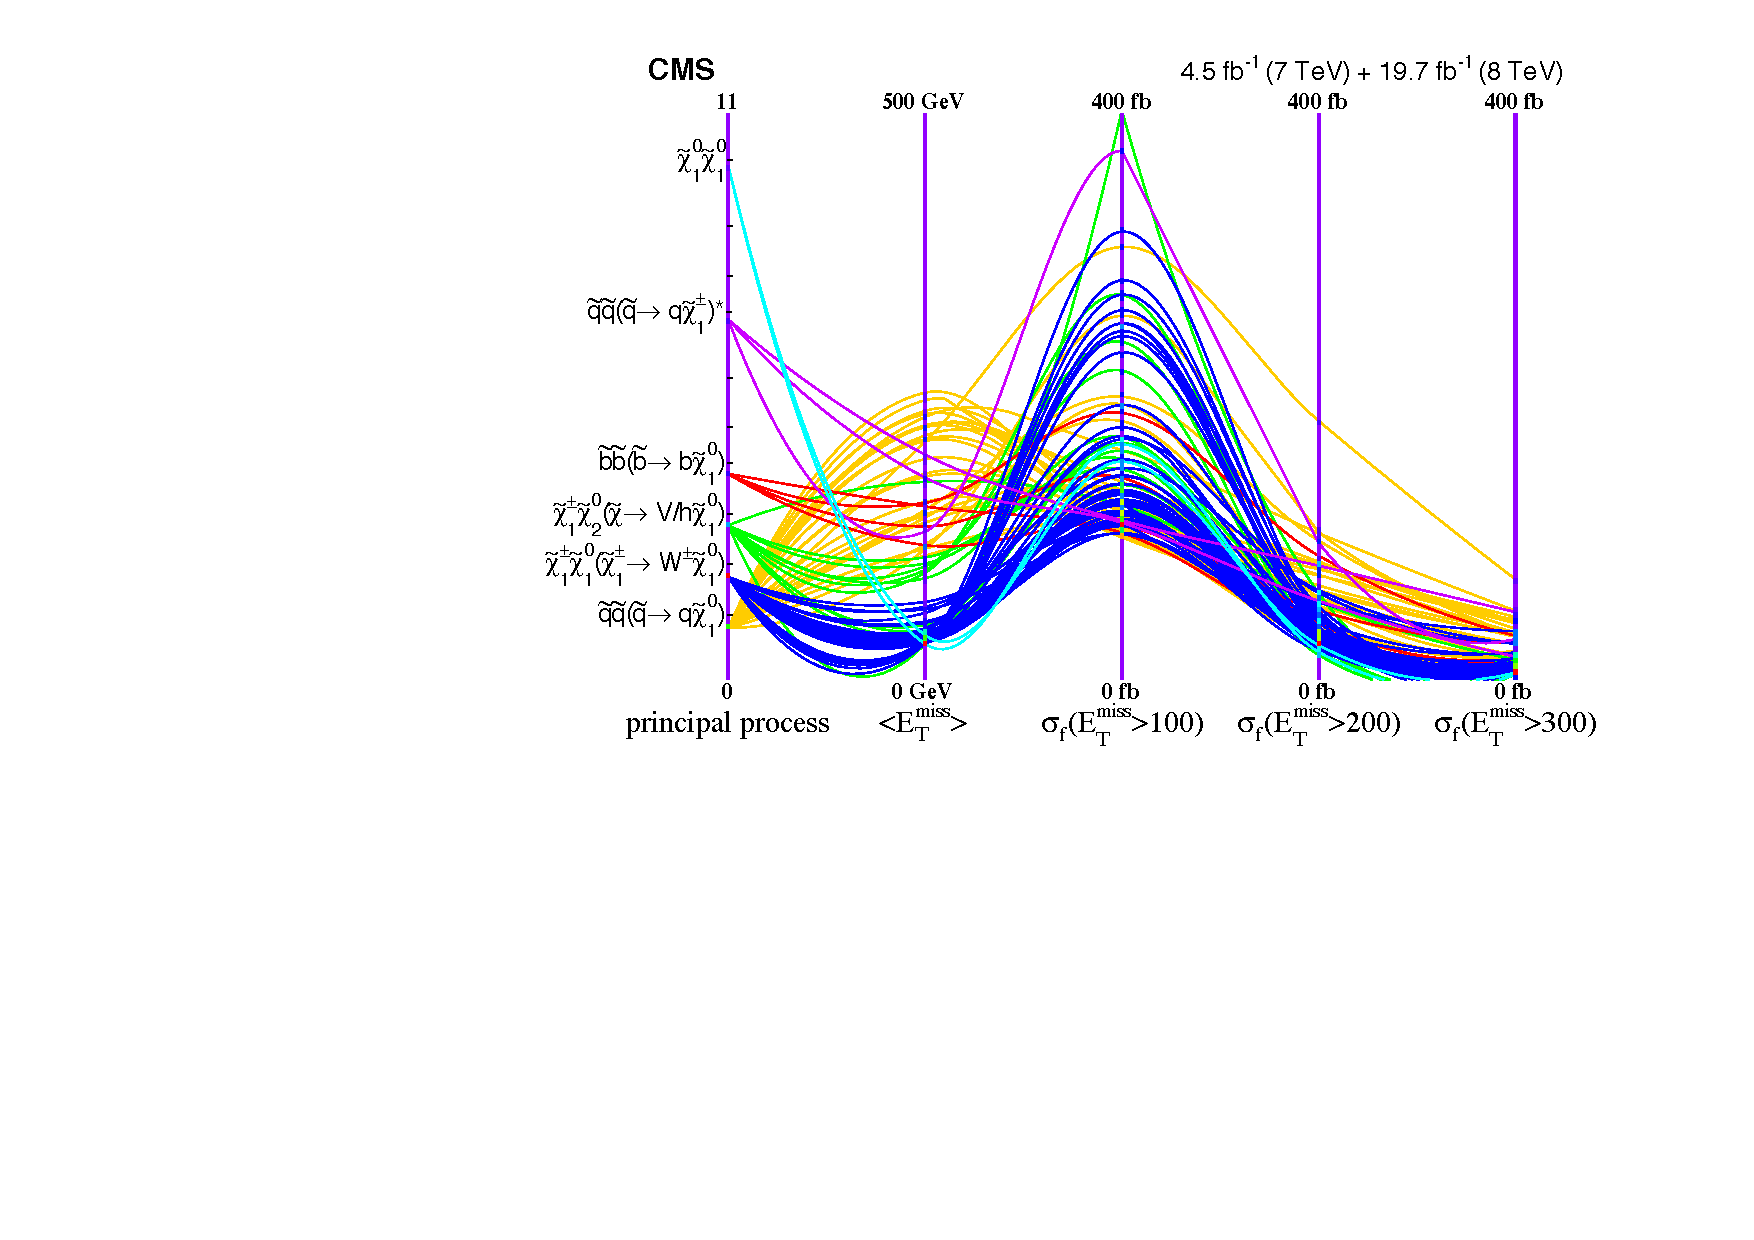
\includegraphics[width=1.0\textwidth]{figures/pMSSMpaper/parallel_coordinates/ParCorToposMET.pdf}
    \caption{A parallel coordinates plot of the nonexcluded pMSSM points
      with the axes set as the principal process, the average \MET{} (in GeV), and the 
    fiducial cross section (in linear scale) for various thresholds on the
    \MET{}. All nonexcluded points corresponding to processes 1, 2, 3,
    4, 7, and 10 that have a fiducial cross section greater than 100 fb are shown. Color is
    assigned to values of the principal process in the same manner as
    in Fig.~\ref{fig:parcor}.}
    \label{fig:parcorMET}
\end{figure}
\begin{figure}[h]
  \centering
         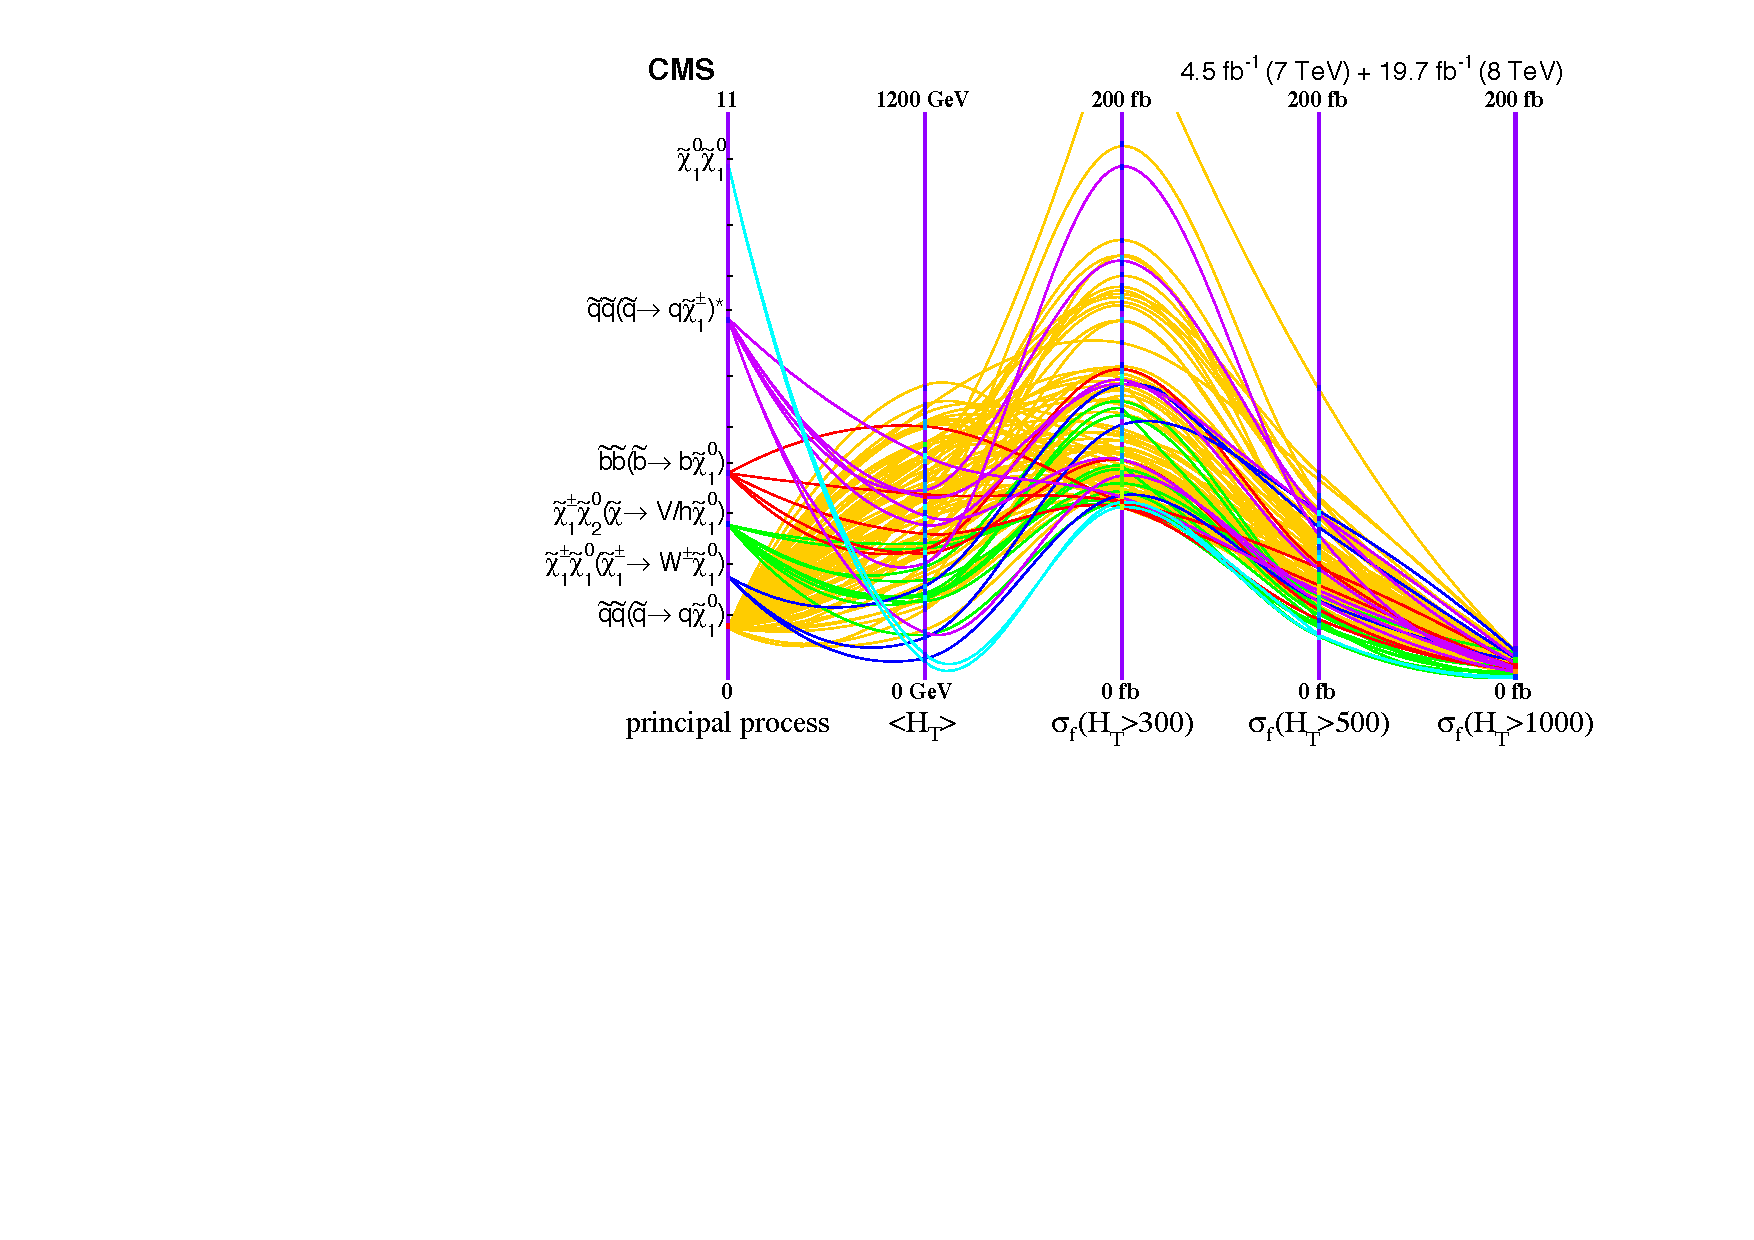
\includegraphics[width=1.0\textwidth]{figures/pMSSMpaper/parallel_coordinates/ParCorToposHT.pdf}
    \caption{A parallel coordinates plot of the nonexcluded pMSSM
      points with the axes set as the principal process, the average
      \HT{} (in GeV), and the 
    fiducial cross section (in linear scale) for various thresholds on the
    \HT{}. All nonexcluded points corresponding to processes 1, 2, 3,
    4, 7, and 10 that have a fiducial cross section greater than
    60 fb
    are shown. Color is assigned to
    values of the principal process in the same manner as in
    Fig.~\ref{fig:parcor}. }
    \label{fig:parcorHT}
\end{figure}
\begin{figure}[h]
  \centering
         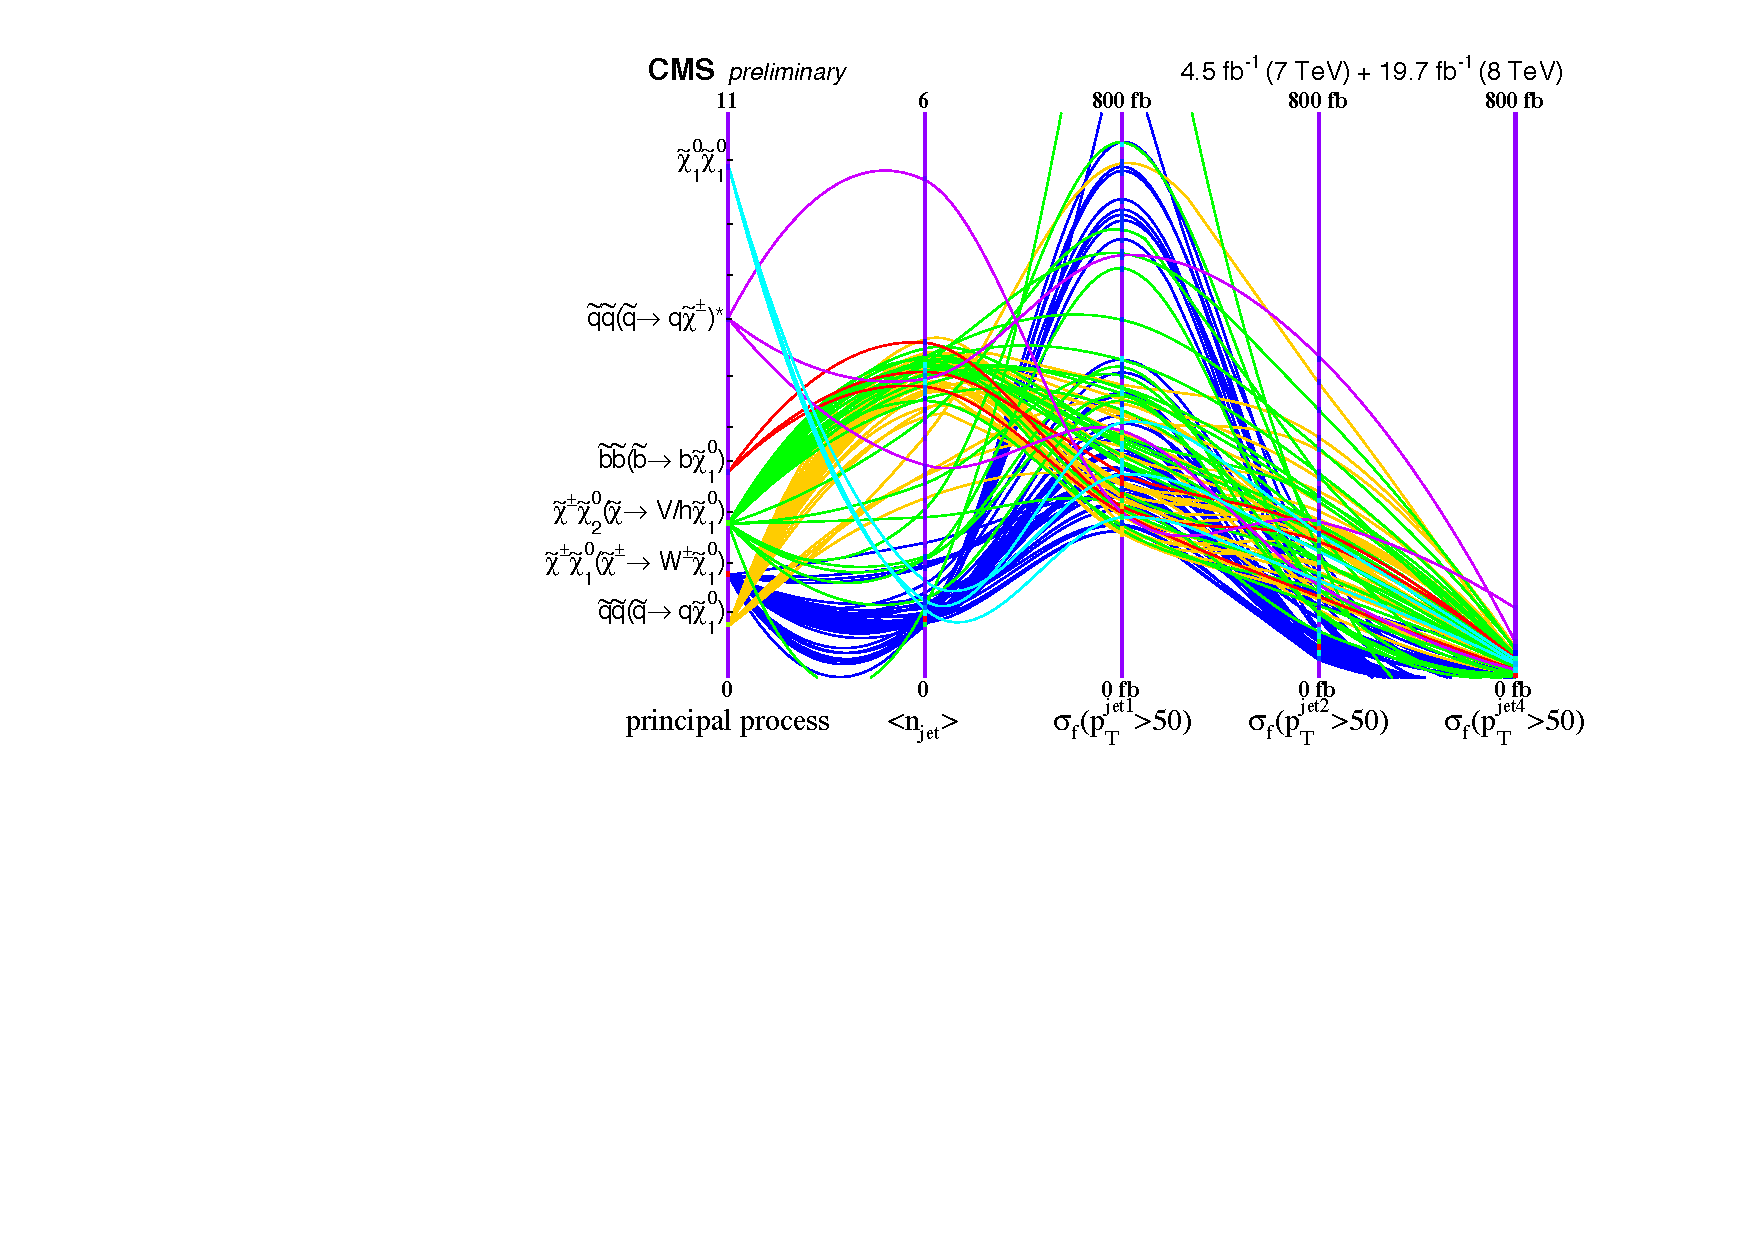
\includegraphics[width=1.0\textwidth]{figures/pMSSMpaper/parallel_coordinates/ParCorToposJets.pdf}
    \caption{A parallel coordinates plot of the nonexcluded pMSSM
      points with the axes set as the principal process and the 
    fiducial cross section (in linear scale) for various thresholds on the
    multiplicity of jets. All nonexcluded points corresponding to processes 1, 2, 3,
    4, 7, and 10 that have a fiducial cross section greater than 200 fb are shown. Color is
    assigned to values of the principal process in the same manner as
    in Fig.~\ref{fig:parcor}. } 
    \label{fig:parcorNJets}
\end{figure}
\begin{figure}[h]
  \centering
   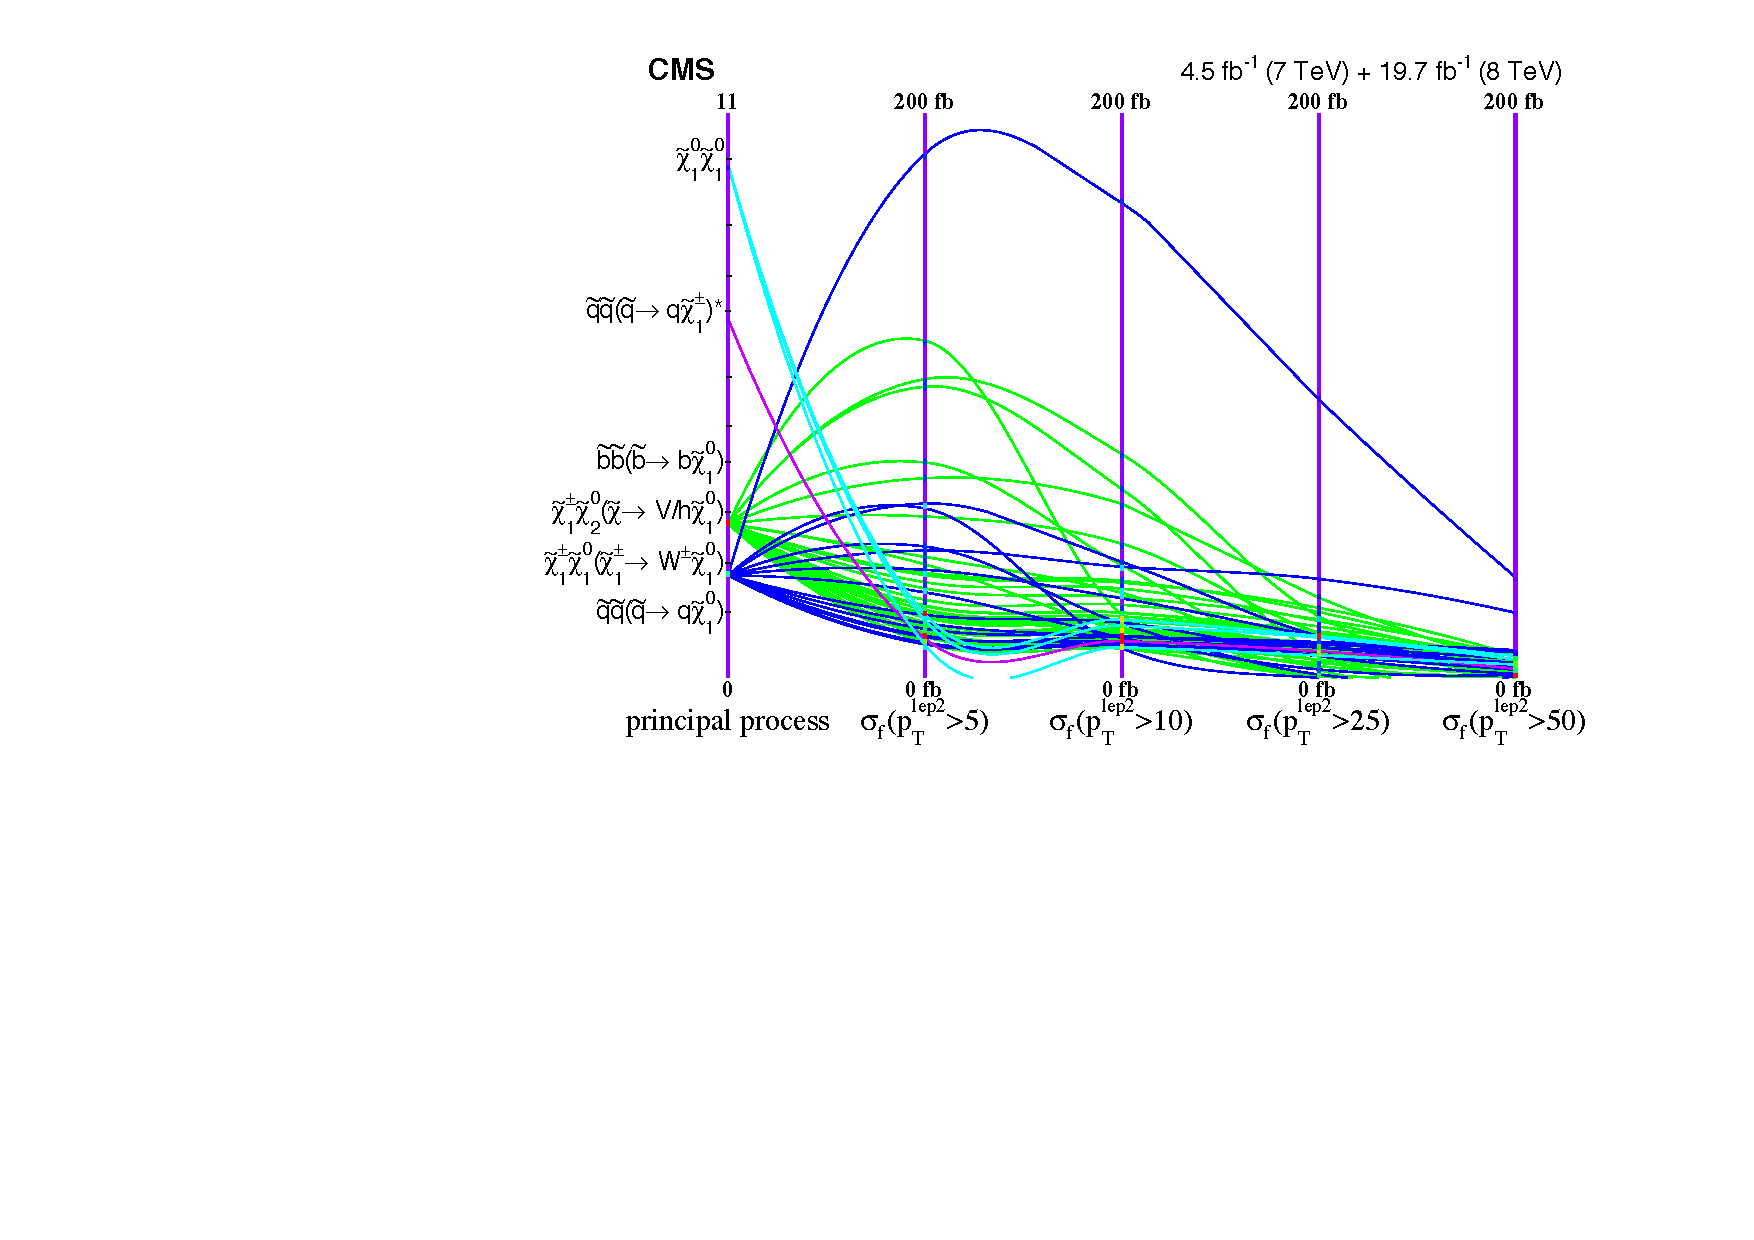
\includegraphics[width=1.0\textwidth]{figures/pMSSMpaper/parallel_coordinates/ParCorToposLep2.pdf}
    \caption{A parallel coordinates plot of the nonexcluded pMSSM
      points with the axes set as the principal process and the 
    fiducial cross section (in linear scale) for various thresholds on the
    sub-leading lepton $p_{\rm T}$ (in GeV). All nonexcluded points corresponding to processes 1, 2, 3,
    4, 7, and 10 that have a fiducial cross section greater than 30 fb are shown. Color is
    assigned to values of the principal process in the same manner as
    in Fig.~\ref{fig:parcor}. } 
    \label{fig:parcorLEP2}
\end{figure}
\begin{figure}[h]
  \centering
   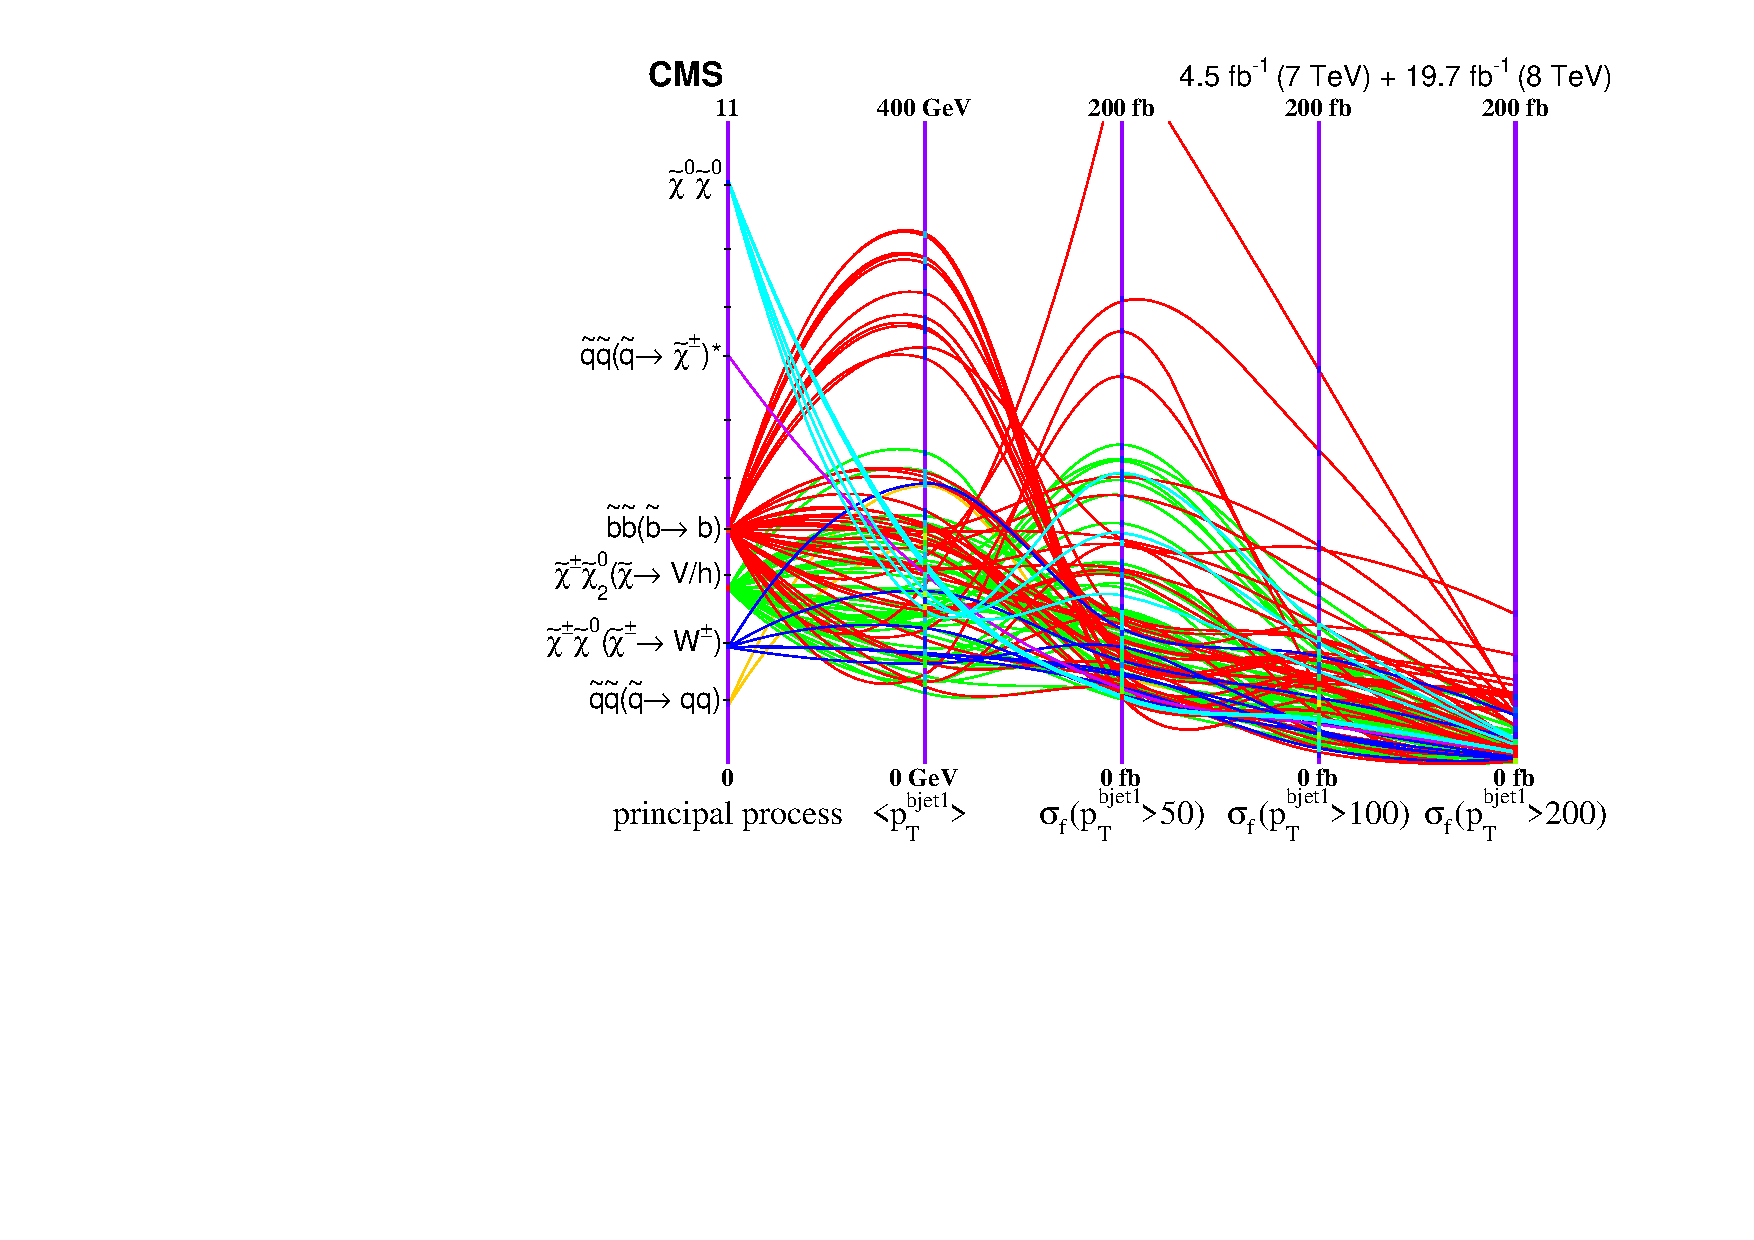
\includegraphics[width=1.0\textwidth]{figures/pMSSMpaper/parallel_coordinates/ParCorToposBjet1.pdf}
    \caption{A parallel coordinates plot of the nonexcluded pMSSM
      points with the axes set as the principal process and the 
    fiducial cross section (in linear scale) for various thresholds on the
    leading b-tagged jet $p_{\rm T}$ (in GeV). All nonexcluded points corresponding to processes 1, 2, 3,
    4, 7, and 10 that have a fiducial cross section greater than 20 fb are shown. Color is
    assigned to values of the principal process in the same manner as
    in Fig.~\ref{fig:parcor}. } 
    \label{fig:parcorBJet1}
\end{figure}

Some principal processes can be associated with large fiducial
cross sections, depending on the final state considered. For example, points with mostly
first-generation squark production give rise to large
fiducial cross sections for events with high \HT{}, resulting in Fig.
\ref{fig:parcorHT} showing mostly orange-colored points; and points with production involving EW gauginos give rise to substantial
fiducial cross sections for events with a high multiplicity of soft leptons, which
explains the unaccompanied blue and green lines in Fig.~\ref{fig:parcorLEP2}.  Somewhat striking is the behavior of the \MET{} fiducial cross section
(Fig.~\ref{fig:parcorMET}), which can increase rapidly (by up to a
factor of ten) as the threshold
is relaxed from 200 to 100 GeV. It is apparent that many of the
nonexcluded regions are not accessible with thresholds of 200 GeV, 
a common criterion applied offline to achieve full efficiency
with the triggers. The fiducial cross section decreases noticeably as the
threshold is further increased from 200 to 300 GeV. Similar behavior is seen for the \HT{} fiducial cross section
(Fig.~\ref{fig:parcorHT}). Fiducial cross
sections are quite large for these final states when a
threshold of 300 GeV is applied, but fall off substantially for higher
thresholds. 

Of course, a loosening of the object thresholds would increase the background yield as well as signal yield. Therefore, a thorough survey of analysis techniques and specific backgrounds will be necessary 
to select optimal values for kinematic thresholds and other analysis techniques to probe the most difficult points. However, the lesson that nonexcluded pMSSM models have large cross sections in background-rich kinematic regions is an open invitation for the development of new techniques that improve signal to background discrimination and background modeling. If the MSSM is realized in one of these difficult regions, the hunt for SUSY will force us to either abandon the LHC, or become more creative. 

